% Pursuing Stacks (cotes 134-2 to 134-8): archive cote 134-4, site page 33 (PDF page 34), typescript page 121.
% typescript. Draft compared: ps3.tex:1628-1694.
% AI-transcribed by Claude Opus 5.5 (claude-opus-5-5, adaptive thinking, effort high), Message Batches API, batch ps2 (msgbatch_01NVwr1Yuo8qJf5rykeGBXPK), 2026-11-12; image review recorded in records/CHECK_DECISIONS_134_3_4.tsv.
\scanpage{134-4/33}
\mspage{121}
if it exists,  and if moreover M has a \uline{strict} initia\over[typed]{h}{l} element, $\hand{\varnothing}_{M}$ .  Re-%
call that $L_{M}$  represents the contravariant functor on M
\[ X \hand{\ensuremath{\longmapsto}} \text{ set of all subobjects of } X \text{ ,} \]
and that the``full'' and ``empty'' subobjects of X,  for variable X,  define
two sections $\hand{\ensuremath{\delta}}_{o}$ and $\hand{\ensuremath{\delta}}_{1}$ of $L_{M}$ .  \over[typed]{E}{I} forgot to state the extra condition that
% NOTE: the right edge of the scan cuts off the ends of several lines (here "tha[t]")
in M fibered products exist (intersection of two subobjects would be
\xout{associative (commutative)}
enough);  then the intersection law endows $L_{M}$ with a structure of a contra\unsure{c}%
% NOTE: line cut off at the right edge after "contra"
tor \inserted[typed]{$\underline{L}_{M}$}, admitting $\hand{\ensuremath{\delta}}_{o}$ as a unit and $\hand{\ensuremath{\delta}}_{1}$ as a zero element.  Moreover,  it is
clear that $L_{M}$ as an interval is separated,  i.e\hand{,} Ker$(\hand{\ensuremath{\delta}}_{o},\hand{\ensuremath{\delta}}_{1}) = \hand{\varnothing}_{M}$ .  M\unsure{\over{e}{o}}re
precisely still,  $L_{M}$ can be viewed as a \uline{final object} \over[typed]{in}{of} \uline{the  category}
\uline{of all} \uline{separated} \uline{intervals in} M,  namely for any such interval,  there is
a \uline{unique} map of intervals
\[ \underline{I} \hand{\ensuremath{\longrightarrow}} L_{M} \text{ .} \]
This implies that if M is endowed with a homotopy structure,  such that
there exists a weak homotopy interval which is separated,  then $\underline{L}_{M}$ is such
an interval,  and it is moreover contractible.\deleted{\xout{and}}  It is doubtful though,
even if we can find a \deleted{\xout{separ}} \uline{generating} contractor for the given homotopy
structure on M,  that the Law\unsure{\over{e}{e}}vere contractor is generating too.

Here now is a second interesting way of getting contractors.  We
assume that M admits finite products (as usual).  Let X be an object,  and
assume the object \uline{Hom}(X,X),  representing the functor
\[ Y \hand{\ensuremath{\longmapsto}} \mathrm{Hom}(X\mathrm{x}Y,X) \ = \ \mathrm{Hom}_{Y}(X_{Y},X_{Y}) \text{ ,} \]
exists in M.  (NB  $X_{Y}$  denotes XxY, viewed as an object of $M_{/Y}$.)\hand{.}  Composi%
% NOTE: line cut off at the right edge after "Composi"
-tion of endomorphisms of $X_{Y}$ clearly endow this functor with an \inserted[typed]{associative} composition
las,  admitting a two-sided unit, which I call $\hand{\ensuremath{e}}_{o}$ .  \xout{(NB} Notice that
sections of \xout{\unsure{Hom $\underline{I}=$}}
\[ \underline{I} = \underline{\mathrm{Hom}}(X,X) \]
can be identified with maps X \hand{$\rightarrow$} X,  and the section corresponding to id$_{X}$
is of course the two-sided unit.  On the other hand,  if X admits sections
% NOTE: line cut off at the right edge after "sections"
i.e. admits ``constant'' endomorphisms,  it is clear that the corresponding
sections of \underline{I} are \xout{right} left zero elements.  If we choose \xout{such} a section\xout{\unsure{,}}
of X,  \underline{I}  becomes a contractor.  It's interest lies in the following

\uline{Proposition}  Assume \xout{xx} finite products exist in M,  and M endowed with
a homotopy structure  \deleted{of type Hom\hand{$_{3}$}  (a weak homotopy interval structure)}.
\margin{\diagram{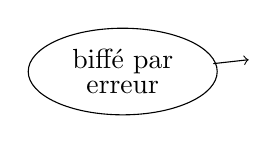
\begin{tikzpicture}[x=1cm,y=1cm,baseline]\draw (0,0) ellipse (1.2 and 0.55);\node at (0,0) {\shortstack{biffé par\\erreur}};\draw[->] (1.15,0.1)--(1.6,0.15);\end{tikzpicture}}} Let X be an object of M endowed with a section $o_{X}$ ,  and suppose \over[typed]{t}{T}he
object \uline{Hom}(X,X) exists,  hence a contractor \underline{I} as seen above.  The follo\unsure{\over{w}{w}}-%
wing \inserted{two} conditions are equivalent:

a)  X is contractible

b)  \underline{I} is contractible (or,  equivalently as seen above\hand{,} \underline{I} is a we\over{a}{a}k
homotopy interval, namely the two endpoints are homotopic).

\margin{33}
